\lecture{15}{31. Marts 2025}{Phase diagrams, Pt. 1}

\section{Phase diagrams}
A phase diagram is a simple diagram showcasing which \textit{phase} a material will be in at a given combination of two of temperature, pressure and combination. 

\subsection{Solubility limit}
For many alloy systems and at some specific temperature, there is a maximum concentration of solute atoms that may dissolve in the solvent to form a solid solution; this is called a \textit{solubility limit}. The addition of solute in excess of this solubility limit results in the formation of another solid solution or compound that has a distinctly different composition. E.g. for the addition of sugar to water, first a syrup forms. As more sugar is introduced, the solution becomes more concentrated, until the solubility limit is reached or the solution becomes saturated with sugar. At this time the solution is not capable of dissolving more sugar, and further additions will simply settle to the bottom. Therefore the system now consists of two separate substances: A sugar-water syrup liquid solution and solid crystals of undissolved sugar.

This solubility limit depends on the temperature of the system. It can be represented in graphical form on a plot of temperature vs. composition. This is shown for sugar in water on \textbf{\autoref{fig:f14_1}}. The solubility limit is the nearly vertical line in the figure. For compositions and temperatures to the left of the solubility limit only the syrup-phase exists. For systems on the right of the solubility limit, solid sugar will settle to the bottom. 
\begin{figure} [ht]
  \centering
  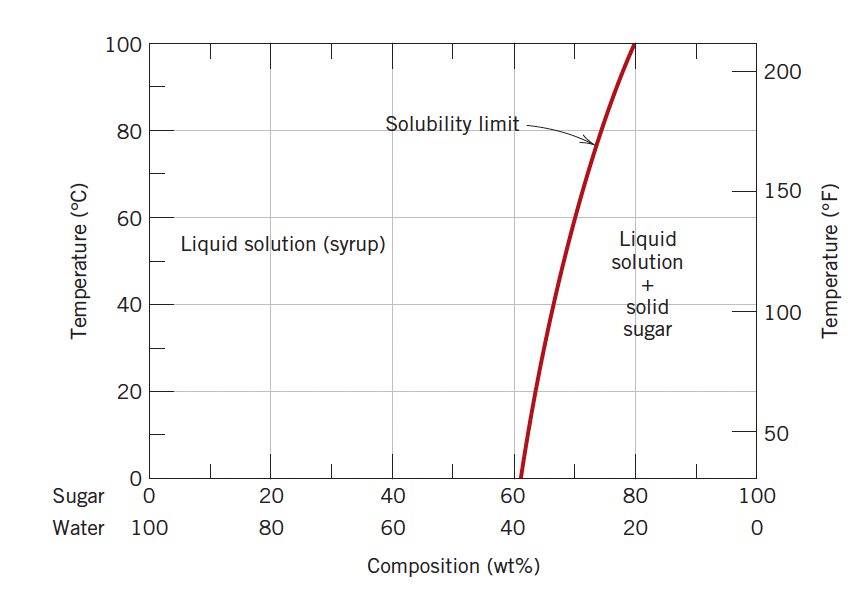
\includegraphics[width=0.5\linewidth]{./figures/f14_1.png}
  \caption{Solubility limit of sugar in water}
  \label{fig:f14_1}
\end{figure}

\subsection{Phases}
Another critical term when talking about phase diagrams is the concept of a \textit{phase}.
\begin{definition}[Phases]
  A phase is a homogeneous portion of a system that has uniform physical and chemical characteristics.
\end{definition}
 Every pure material is considered to be a phase; so also is every solid, liquid, and gaseous solution. E.g. the water-sugar syrup phase disussed before is a phase and so is solid sugar. Each phase has different physical properties (one is a liquid and the other is a solid in the aforementioned example). Furthermore, each is chemically different (i.e. the different chemical compositiions of water and sugar in the aforementioned example). If more than one phase if present in a given system, each will have its own distinct properties, and a boundary separating the phases will exist, across which there will be a discontinuous and abrupt change in physical and/or chemical characteristics.

Sometimes, a single-phase system is termed \textit{homogeneous}. Systems composed of two or more phases, are termed \textit{mixtures} or \textit{heterogeneous systems}. Most metalic alloys and, for that matter, ceramic, polymeric, and composite systems are heterogeneous. Typically, the phases interact in such a way that the property combination of the multiphase system is different from, and more desirable than, either of the individual phases.


\subsection{Microstructure}
The physical properties and, in particular, the mechanical properties of a material often depend on the microstructure. Microstructure is subjected to direct microscopic observation using optical or electron microscopes. In metal alloys, microstructure is characterized by the number of phases present, their proportions, and the manner in which they are distributed or arranged. The microstructure of an alloy depends on such variables as the alloying elements present, their concentrations, and the heat treatment of the alloy). 

\subsection{Phase equilibria}
\textit{Equilibrium} is another essential concept, it is best described in terms of a thermodynamic quantity called the \textit{free energy}. In brief, \textit{free energy} is a function of the internal energy of a system and also the randomness or disorder of the atoms or molecules (the sum of enthalpy and entropy). A system is at equilibrium if its free energy is at a minimum under some specified combination of temperature, pressure, and composition. In a macroscopic sense, this means that the characteristics of the system do not change with time, but persist indefinitely -- that is, the system is stable. A change in temperature, pressure and/or composition for a system in equilibrium results in an increase in the free energy and in a possible spontaneous change to another state by which the free energy is lowered.

The term \textit{phase equilibrium}, often used in the context of this discussion, refers to equilibrium as it applies to systems in which more than one phase may exist. Phase equilibrium is reflected by a constancy with time in the phase characteristics of a system.

It is often the case, especially in solid systems, that a state of equilibrium is never completely achieved because the rate of approach to equilibrium is extremely slow; such a system is said to be in a \textit{nonequilibrium} or \textit{metastable} state. A metastable state or microstructure may persist indefinitely, experiencing only extremely slight and almost imperceptible changes as time progresses. Often, metastable structures are of more practical significance than equilibrium ones. 

\subsection{One-component (unary) phase diagrams}
Much of the information about the control of the phase structure of a particular system is conveniently and concisely displayed in what is called a \textit{phase diagram}, also often termed an equilibrium diagram. Three externally controllable parameters affect phase structure -- temperature, pressure and composition -- and phase diagrams are constructed when various combinations of these parameters are plotted against one another. 

Perhaps the simplest and easiest type of phase diagram to understand is that for a one-component system, in which composition is held constant (i.e., the phase diagram is for a pure substance); this means that pressure and temperature are the variables. This one-component phase diagram is represented as a two-dimensional plot of pressure versus temperature. Most often the pressure axis is scaled logarithmically.

On \textbf{\autoref{fig:f14_2}} a phase diagram for pure water is shown. Regions for three different phases -- solid, liquid, and vapor -- are delineated on the plot. Each pf the phases exist under equilibrium conditions over the temperature-pressure ranges of its corresponding area. 

\begin{figure} [ht]
  \centering
  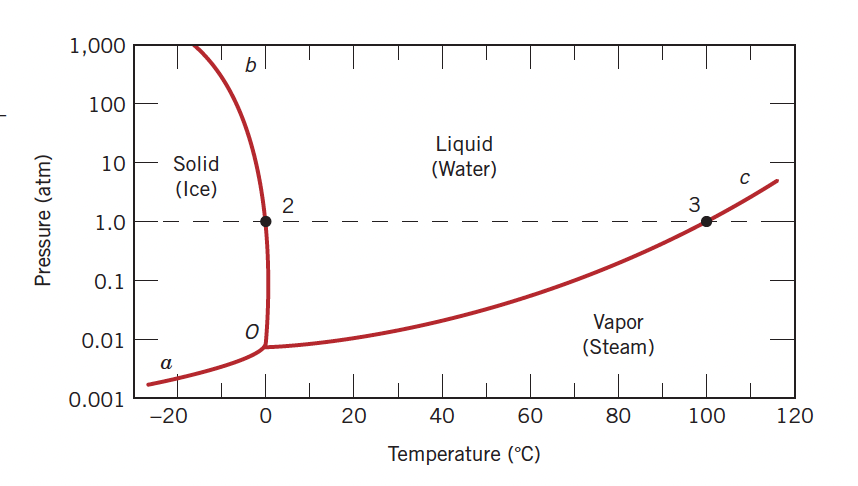
\includegraphics[width=0.5\linewidth]{./figures/f14_2.png}
  \caption{Phase diagram for pure water}
  \label{fig:f14_2}
\end{figure}


\subsection{Binary phase diagrams}
Another type of extremely common phase diagram is one in which temperature and composition are variable parameters and pressure is held constant -- normally \qty{1}{atm}. There are several different varieties; in the present discussion, we will concern ourselves with binary alloys. If more than two components are present, phase diagrams become extremely complicated and difficult to represent. An explanation of the principles governing and the interpretation of phase diagrams can be demonstrated using binary alloys even though most alloys contain more than two components.

Binary phase diagrams are maps that represent the relationships between temperature and the compositions and quantities of phases at equilibrium, which influence the microstructure of an allow. Many microstructures develop from \textit{phase transformations}; the changes that occur when the temperature is altered. This may involve the transition from one phase to another or the appearance or disappearance of a phase. 


\subsection{Binary isomorphous systems}
Possibly the easiest type of binary phase diagram to understand and interpret is the type that is characterized by the copper-nickel system shown on \textbf{\autoref{fig:f14_3}}. The composition ranges from \qty{0}{wt}\% Ni (\qty{100}{wt}\%) on the har left and \qty{100}{wt}\% Ni (\qty{0}{wt}\% Cu) on the right Three different phase regions, or \textit{fields}, appear on the diagram: An alpha ($\alpha$) field, a liquid ($L$) field, and a two-phase $\alpha+L$ field. Each reqion is defined by the phase or phases that exits over the range of temperatures and compositions delineated by the phase boundary lines.

\begin{figure} [ht]
  \centering
  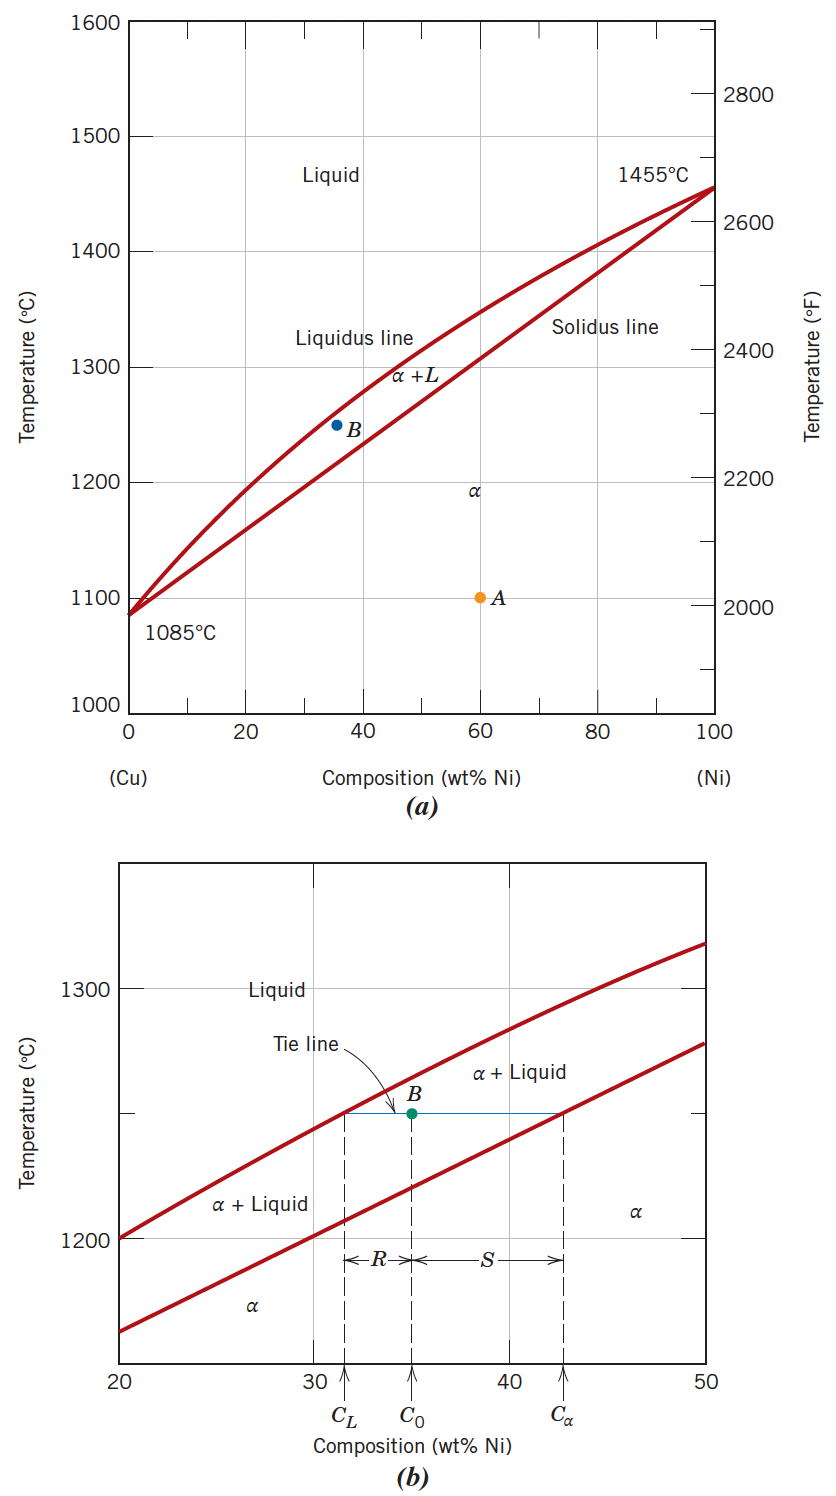
\includegraphics[width=0.25\linewidth]{./figures/f14_3.png}
  \caption{Copper-nickel phase diagram}
  \label{fig:f14_3}
\end{figure}

The liquid $L$ is a homogeneous liquid solution compound of both copper and nickel. The $\alpha$ phase is a substitutional solid solution consisting of both Cu and Ni atoms and has an FCC crystal structure. At temperatures below about \qty{1080}{\celsius}, copper and nickel are mutually soluble in each other in the solid state for all compositions. This complete solubility is explained by the fact that both Cu and Ni have the same crystal structure, nearly identical atomic radii and electronegativities, and similar valences. Therefore the copper-nickel system is termed \textit{isomorphous} because of the complete liquid and solid solubility of the two components.

For metallic alloys, solid solutions are commonly designated by lowercase Greek letters ($\alpha, \beta, \gamma$, etc.). With regard to phase boundaries, the line separating the $L$ and $\alpha + L$ phase fields is termed the \textit{liquidus line}. The \textit{solidus line} is located between the $\alpha$ and $\alpha + L$ regions. On \textbf{\autoref{fig:f14_3}} the \textit{liquidus} and \textit{solidus} lines intersect at the two composition extremes; these correspond to the melting temperatures of the pure components. For any temperature between these two extremes the solid-to-liquid transformation takes place at the melting temperature, meaning some of the heat energy will be stored as latent energy over this interval (in this way the interval corresponds to the single melting temperature of a pure substance).

\subsection{Interpretation of phase diagrams}
For a binary system of known composition and temperature at equilibrium, at least three kinds of information are available:
\begin{enumerate}
  \item The phases that are present
  \item The compositions of these phases
  \item The percentages or fractions of the phases
\end{enumerate}


\subsubsection{Phases present}
The establishment of what phases are present is relatively simple. One just locates the temperature-composition point on the diagram and notes the phase(s) with which the corresponding phase field is labeled.

\subsubsection{Determination of phase compositions}
The first step in the determination of phase compositions (in terms of the concentrations of the components) is to locate the temperature-composition point on the phase diagram. Different methods are used for single- and two-phase regions. If only one phase is present the procedure is trivial: The composition of this phase is simple the same as the overall composition of the alloy.

For an alloy having a composition and temperature located in a two-phase region, the situation is more complicated. In all two-phase regions (and in two-phase regions only), one may imagine a series of horizontal lines, one at every temperature; each of these is known as a \textit{tie line}, or sometimes an \textit{isotherm}. These tie lines extend across the two-phase reqion and terminate at the phase boundary lines on either side. To compute the equilibrium concentrations of the two phases, the following procedure is used:
\begin{enumerate}
  \item A tie line is constructed across the two-phase reqion at the temperature of the alloy
  \item The intersections of the tie line and the phase boundaries on either side are noted
  \item Perpendiculars are dropped from these intersections to the horizontal composition axis, from which the composition of each of the respective phases is read. 
\end{enumerate}


\subsubsection{Determination of phase amounts}
The relative amounts (as fractions or as percentages) of the phases present at equilibrium may also be computed with the aid of phase diagrams. Again, the single- and two-phase situations must be treated separately. The solution is obvious in the single-phase region. Because only one phase is present, the alloy is composed entirely of that phase -- that is, the phase fraction is \num{1,0}.

If the composition and temperature position is located within a two-phase region, things are more complex. The tie line must be used in conjunction with a procedure that is often called the \textit{lever rule} (or the \textit{inverse lever rule}), which is applied as:
\begin{enumerate}
  \item The tie line is constructed across the two-phase region at the temperature of the alloy
  \item The overall composition is located on the tie line
  \item The fraction of one phase is computed by taking the length of tie line from the overall alloy composition on the phase boundary for the \textit{other phase} and dividing by the total tie line length.
  \item The fraction of the other phase is determined in the same manner
  \item If phase percentages are desired, each phase fraction is multiplied by 100. When the composition axis is scaled in weight percent, the phase fractions computed using the lever rule are \textit{mass fractions} -- the mass (or weight) of a specified phase divided by the total alloy mass (or weight). The mass of each phase is computed from the product of each phase fraction and the total alloy mass.
\end{enumerate}
In the use of the lever rule, tie line segment lengths may be determined either by direct measurement from the phase diagram using a ruler, or by subtracting compositions as taken from the composition axis.

The lever rule is therefore
\[ 
W_L = \frac{S}{R + S} = \frac{C_{\alpha} - C_0}{C_{\alpha} - C_L}
.\]

For multiphase alloys, it is often more convenient to specify relative phase amount in terms of volume fractions rather than mass fractions. Phase volume fractions are preferred because they may be determined from examination of the microstructure; furthermore, the properties of a multiphase alloy is better described by volume fractions than mass fractions. For an alloy consisting of $\alpha$ and $\beta$ phases, the volume fraction of the $\alpha$ phase, $V_{\alpha}$ is defined as:
\[ 
V_{\alpha} = \frac{v_{\alpha}}{v_{\alpha} + v_{\beta}}
\]
where $v_{\alpha}$ and $v_{\beta}$ denote the volumes of the respective phases in the alloy. An analogous expression exists for $V_{\beta}$, and, for an alloy consisting of just two phases, it is the case that $V_{\alpha} + V_{\beta} = 1$. 

To convert between volume and mass fractions one can simply scale by the density of the relevant phase as:
\begin{align*}
  V_{\alpha} &= \frac{\frac{W_{\alpha}}{\rho_{\alpha}}}{\frac{W_{\alpha}}{\rho_{\alpha}} + \frac{W_{\beta}}{\rho_{\beta}}} \\
  W_{\alpha} &= \frac{V_{\alpha} \rho_{\alpha}}{V_{\alpha}\rho_{\alpha} + V_{\beta} \rho_{\beta}}
.\end{align*}


\subsection{Development of microstructure in isomophous alloys}

\subsubsection{Equilibrium Cooling}
At this point it is instructive to examine the development of microstructures that occurs for isomorphous alloys during solidification. We first treat the situation in which the cooling occurs very slowly and where phase equilibrium is continuously maintained. As cooling begins, no microstructural or compositional changes will be realized until we reach the liquidus line. At this point, the first solid state begins to form (for copper-nickel the $\alpha$ phase will start forming), with a composition dictated by the tie line drawn at this temperature. With continued cooling, both compositions of the liquid and $\alpha$ phases will follow the liquidus and solidus lines, respectively.


\subsubsection{Nonequilibrium cooling}
Conditions of equilibrium solidification and the development of microstructures as described in the previous section, are realized only for extremely slow cooling rates. The reason for this is that with changes in temperature, there must be readjustments in the compositions of the liquid and solid phases in accordance with the phase diagram (i.e., the liquidus and solidus lines). These readjustments are accomplished by diffusional processes -- that is, diffusion in both solid and liquid phases and also across the solid-liquid interface. Because diffusion is a time-dependent phenomenon, to maintain equilibrium during cooling, sufficient time must be allowed at each temperature to allow for the appropriate compositional readjustments. Diffusion rates are especially low for the solid phase, and for both phases, decrease with temperature. In virtually all practical solidification situations, cooling rates are much too rapid to allow these compositional readjustments and maintenance of equilibrium. Therefore other microstructures often develop.

There are some important consequences for isomorphous alloys that have solidified under nonequilibrium conditions. The distribution of the two elements within the grains will e.g. be nonuniform. A phenomenon called \textit{segregation} -- that is, concentration gradients are established across the grains. The center of each grain, which is the first part to freeze is rich in the high-melting element, whereas the concentration of the low-melting element increases with position from this region to the grain boundary. This is termed a \textit{cored} structure, which gives rise to less than the optimal properties. As a casting having a cored structure is reheated, grain boundary regions melt first because they are rich in the low-melting component. This produces a sudden loss in mechanical integrity due to the thin liquid film that separates the grains. Furthermore, this melting may begin at a temperature below the euilibrium solidus temperature of the alloy. Coring may be eliminated by a homogenization heat treatment carried out at a temperature below the solidus point for the particular alloy composition. During this process, atomic diffusion occurs, which produces compositionally homogeneous grains.


\subsection{Mechanical properties of isomorphous alloys}
For all temperature and compositions below the melting temperature of the lowest-melting component, only a single solid phase exists. Therefore, each component experiences solid-solution strengthening.


\subsection{Binary eutectuc systems}
Another type of common and relatively simple phase diagram found for binary alloys is shown on \textbf{\autoref{fig:f14_4}} -- this is a \textit{binary eutectic phase diagram}. A number of features of this phase diagram are important and worth noting. First, three single-phase regions are found on the diagram: $\alpha$, $\beta$ and liquid. The $\alpha$ phase is a solid solution rich in copper; it has silver as the solute component and an FCC crystal structure. The $\beta$ phase solid solution also has an FCC structure, but copper is the solute. Pure copper and pure silver are also considered to be $\alpha$ and $\beta$ phases, respectively. 

\begin{figure} [ht]
  \centering
  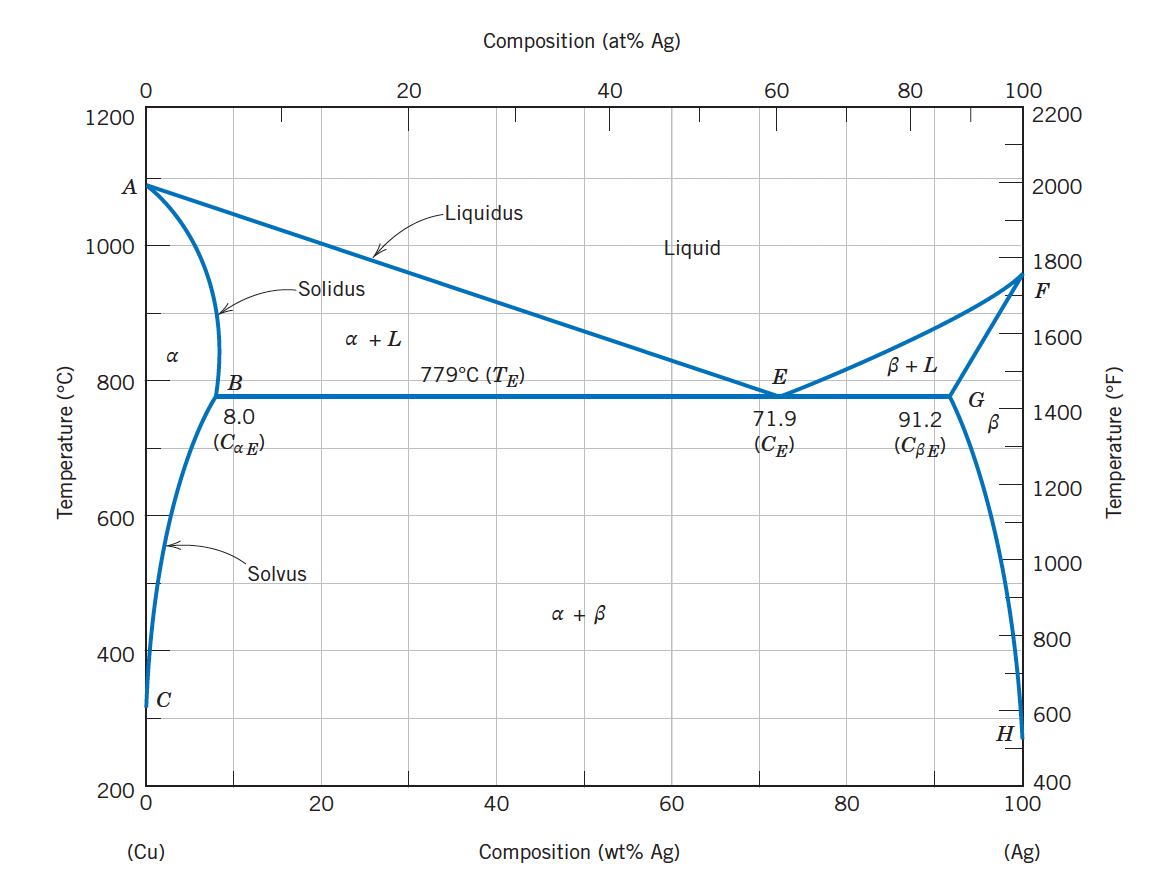
\includegraphics[width=0.5\linewidth]{./figures/f14_4.png}
  \caption{Copper-silver phase diagram}
  \label{fig:f14_4}
\end{figure}

The solubility in each of these solid phases is limited, in that at any temperature below line $BEG$ on \textbf{\autoref{fig:f14_4}} only a limited concentration of silver dissolves in copper (for the $\alpha$ phase), and similarly for copper in silver (the $\beta$ phase). The solubility limit for the $\alpha$ phase corresponds to the boundary line, labeled $CBA$, between the $\frac{\alpha}{\alpha + \beta}$ and $\frac{\alpha}{\alpha + L}$ phase regions. At temperatures below \qty{779}{\celsius}, the solid solubility limit line separating the $\alpha$ and $\alpha + \beta$ phase regions is termed a \textit{solvus line}; the boundary $AB$ is the \textit{solidus line}.

As silver is added to copper, the temperature at which the alloys become totally liquid decreases along the \textit{liquidus line}, $AE$; thus, the melting temperature of copper is lowered by silver additions. The same may be said for silver: THe introduction of copper reduces the temperature of complete melting along the other liquidus line, $FE$. These liquidus lines meet at point $E$ on the phase diagram, with composition $C_E$ and temperature $T_E$. It should be noted that there is a horizontal isotherm at \qty{779}{\celsius} and represented by the line labelled $BEG$ that also passes through point $E$.

An important reaction occurs for an alloy of composition $C_E$ as it changes temperature in passing through $T_E$; this reaction may be written as
\[ 
L(C_E) {\rightleftharpoons} \alpha(C_{\alpha E}) + \beta(C_{\beta E})
.\]

Or, upon cooling, a liquid phase is transformed into the two solid $\alpha$ and $\beta$ phases at the temperature $T_E$. The opposite reaction occurs upon heating. This is called a \textit{eutectic reaction} (\textit{eutectic} means ``easily melted''), and point $E$ on the diagram is called the \textit{eutectic point}; furthermore, $C_E$ and $T_E$ represent the eutectuc composition and temperature, respectively. The eutectic reaction above for silver and copper may be written as
\[ 
L(\qty{71,9}{wt}\% \text{ Ag}) \leftrightharpoons \alpha(\qty{8,0}{wt}\% \text{ Ag}) + \beta(\qty{91,2}{wt}\% \text{ Ag})
.\]
This eutectic reaction is termed an \textit{invariant reaction} insomuch as it occurs under equilibrium conditions at a specific temperature ($T_E$) and specific compositions ($C_E$, $C_{\alpha E}$ and $C_{\beta E}$), which are constant (i.e., invariable) for a specific binary system. Furthermore, the horizontal solidus line $BEG$ at $T_E$ is sometimes called the \textit{eutectic isotherm}.

The eutectic reaction, upon cooling, is similar to solidification for pure components in that the reaction proceeds to completion at a constant temperature, or \textit{isothermally}, at $T_E$. However, the solid product of eutectic solidification is always two solid phases, whereas for a pure component only a single phase forms. Because of this eutectic reaction, phase diagrams similar to \textbf{\autoref{fig:f14_4}} ater termed \textit{eutectuc phase diagrams}; components exhibiting this behaviour make up a \textit{eutectic system}. 
